\documentclass[a4paper,11pt,fleqn,twoside,openright,oldfontcommand]{memoir} 	% Openright aabner kapitler paa hoejresider (openany begge)

%%%% PAKKER %%%%

% ¤¤ Oversaettelse og tegnsaetning ¤¤ %
\usepackage[utf8]{inputenc}					% Input-indkodning af tegnsaet (UTF8)
\usepackage[danish]{babel}					% Dokumentets sprog
\usepackage[T1]{fontenc}					% Output-indkodning af tegnsaet (T1)
\usepackage{ragged2e,anyfontsize}			% Justering af elementer
\usepackage{fixltx2e}						% Retter forskellige fejl i LaTeX-kernen
			
																
% ¤¤ Figurer og tabeller (floats) ¤¤ %
\usepackage{graphicx} 						% Haandtering af eksterne billeder (JPG, PNG, PDF)
\usepackage{multirow}                		% Fletning af raekker og kolonner (\multicolumn og \multirow)
\usepackage{colortbl} 						% Farver i tabeller (fx \columncolor, \rowcolor og \cellcolor)
\usepackage[dvipsnames]{xcolor}				% Definer farver med \definecolor. Se mere: http://en.wikibooks.org/wiki/LaTeX/Colors
\usepackage{flafter}						% Soerger for at floats ikke optraeder i teksten foer deres reference
\let\newfloat\relax 						% Justering mellem float-pakken og memoir
\usepackage{float}							% Muliggoer eksakt placering af floats, f.eks. \begin{figure}[H]
%\usepackage{eso-pic}						% Tilfoej billedekommandoer paa hver side
%\usepackage{wrapfig}						% Indsaettelse af figurer omsvoebt af tekst. \begin{wrapfigure}{Placering}{Stoerrelse}
%\usepackage{multicol}         	        	% Muliggoer tekst i spalter
%\usepackage{rotating}						% Rotation af tekst med \begin{sideways}...\end{sideways}

% ¤¤ Matematik mm. ¤¤
\usepackage{amsmath,amssymb,stmaryrd} 		% Avancerede matematik-udvidelser
\usepackage{mathtools}						% Andre matematik- og tegnudvidelser
\usepackage{textcomp}                 		% Symbol-udvidelser (f.eks. promille-tegn med \textperthousand )
\usepackage{siunitx}						% Flot og konsistent praesentation af tal og enheder med \si{enhed} og \SI{tal}{enhed}
\sisetup{output-decimal-marker = {,}}		% Opsaetning af \SI (DE for komma som decimalseparator) 
\usepackage[version=3]{mhchem} 				% Kemi-pakke til flot og let notation af formler, f.eks. \ce{Fe2O3}
%\usepackage{rsphrase}						% Kemi-pakke til RS-saetninger, f.eks. \rsphrase{R1}

% ¤¤ Referencer og kilder ¤¤ %
\usepackage[danish]{varioref}				% Muliggoer bl.a. krydshenvisninger med sidetal (\vref)
\usepackage[numbers,sort&compress]{natbib}

% ¤¤ Misc. ¤¤ %
\usepackage{listings}						% Placer kildekode i dokumentet med \begin{lstlisting}...\end{lstlisting}
\usepackage{lipsum}							% Dummy text \lipsum[..]
\usepackage[shortlabels]{enumitem}			% Muliggoer enkelt konfiguration af lister
\usepackage{pdfpages}						% Goer det muligt at inkludere pdf-dokumenter med kommandoen \includepdf[pages={x-y}]{fil.pdf}	
\pdfoptionpdfminorversion=6					% Muliggoer inkludering af pdf dokumenter, af version 1.6 og hoejere
\pretolerance=2500 							% Justering af afstand mellem ord (hoejt tal, mindre orddeling og mere luft mellem ord)
\usepackage{geometry}
\usepackage{titlesec}  						%needs recent version of »titlesec«
\usepackage{xcolor}

% Kommentarer og rettelser med \fxnote. Med 'final' i stedet for 'draft' udloeser hver note en error i den faerdige rapport.
\usepackage[footnote,draft,danish,silent,nomargin]{fixme}		


%%%% BRUGERDEFINEREDE INDSTILLINGER %%%%

% ¤¤ Marginer ¤¤ %
\setlrmarginsandblock{3.0cm}{3.0cm}{*}		% \setlrmarginsandblock{Indbinding}{Kant}{Ratio}
\setulmarginsandblock{3.0cm}{3.0cm}{*}		% \setulmarginsandblock{Top}{Bund}{Ratio}
\checkandfixthelayout 						% Oversaetter vaerdier til brug for andre pakker

%	¤¤ Afsnitsformatering ¤¤ %
\setlength{\parindent}{0mm}           		% Stoerrelse af indryk
\setlength{\parskip}{3mm}          			% Afstand mellem afsnit ved brug af double Enter
\linespread{1,1}							% Linie afstand

% ¤¤ Litteraturlisten ¤¤ %
\bibliographystyle{unsrtnat}

% ¤¤ Indholdsfortegnelse ¤¤ %
\setsecnumdepth{subsection}		 			% Dybden af nummerede overkrifter (part/chapter/section/subsection)
\maxsecnumdepth{subsection}					% Dokumentklassens graense for nummereringsdybde
\settocdepth{subsection} 					% Dybden af indholdsfortegnelsen

% ¤¤ Lister ¤¤ %
\setlist{
  topsep=0pt,								% Vertikal afstand mellem tekst og listen
  itemsep=-1ex,								% Vertikal afstand mellem items
} 

% ¤¤ Visuelle referencer ¤¤ %
\usepackage[colorlinks]{hyperref}			% Danner klikbare referencer (hyperlinks) i dokumentet.
\hypersetup{colorlinks = true,				% Opsaetning af farvede hyperlinks (interne links, citeringer og URL)
    linkcolor = black,
    citecolor = black,
    urlcolor = black
}

% ¤¤ Opsaetning af figur- og tabeltekst ¤¤ %
\captionnamefont{\small\bfseries\itshape}	% Opsaetning af tekstdelen ('Figur' eller 'Tabel')
\captiontitlefont{\small}					% Opsaetning af nummerering
\captiondelim{. }							% Seperator mellem nummerering og figurtekst
\hangcaption								% Venstrejusterer flere-liniers figurtekst under hinanden
\captionwidth{\linewidth}					% Bredden af figurteksten
\setlength{\belowcaptionskip}{0pt}			% Afstand under figurteksten
		
% ¤¤ Opsaetning af listings ¤¤ %
\definecolor{commentGreen}{RGB}{34,139,24}
\definecolor{stringPurple}{RGB}{208,76,239}

\lstset{language=Matlab,					% Sprog
	basicstyle=\ttfamily\scriptsize,		% Opsaetning af teksten
	keywords={for,if,while,else,elseif,		% Noegleord at fremhaeve
			  end,break,return,case,
			  switch,function},
	keywordstyle=\color{blue},				% Opsaetning af noegleord
	commentstyle=\color{commentGreen},		% Opsaetning af kommentarer
	stringstyle=\color{stringPurple},		% Opsaetning af strenge
	showstringspaces=false,					% Mellemrum i strenge enten vist eller blanke
	numbers=left, numberstyle=\tiny,		% Linjenumre
	extendedchars=true, 					% Tillader specielle karakterer
	columns=flexible,						% Kolonnejustering
	breaklines, breakatwhitespace=true,		% Bryd lange linjer
}

% ¤¤ Navngivning ¤¤ %
\addto\captionsdanish{
	\renewcommand\appendixname{Bilag}
	\renewcommand\contentsname{Indholdsfortegnelse}	
	\renewcommand\appendixpagename{Bilag}
	\renewcommand\appendixtocname{Bilag}
	\renewcommand\cftchaptername{\chaptername~}				% Skriver "Kapitel" foran kapitlerne i indholdsfortegnelsen
	\renewcommand\cftappendixname{\appendixname~}			% Skriver "Appendiks" foran appendiks i indholdsfortegnelsen
}

% ¤¤ Kapiteludssende ¤¤ %
\definecolor{numbercolor}{gray}{0.7}		% Definerer en farve til brug til kapiteludseende
\newif\ifchapternonum

\makechapterstyle{jenor}{					% Definerer kapiteludseende frem til ...
  \renewcommand\beforechapskip{0pt}
  \renewcommand\printchaptername{}
  \renewcommand\printchapternum{}
  \renewcommand\printchapternonum{\chapternonumtrue}
  \renewcommand\chaptitlefont{\fontfamily{pbk}\fontseries{db}\fontshape{n}\fontsize{25}{35}\selectfont\raggedleft}
  \renewcommand\chapnumfont{\fontfamily{pbk}\fontseries{m}\fontshape{n}\fontsize{1in}{0in}\selectfont\color{numbercolor}}
  \renewcommand\printchaptertitle[1]{%
    \noindent
    \ifchapternonum
    \begin{tabularx}{\textwidth}{X}
    {\let\\\newline\chaptitlefont ##1\par} 
    \end{tabularx}
    \par\vskip-2.5mm\hrule
    \else
    \begin{tabularx}{\textwidth}{Xl}
    {\parbox[b]{\linewidth}{\chaptitlefont ##1}} & \raisebox{-15pt}{\chapnumfont \thechapter}
    \end{tabularx}
    \par\vskip2mm\hrule
    \fi
  }
}											% ... her

\chapterstyle{jenor}						% Valg af kapiteludseende - Google 'memoir chapter styles' for alternativer

% ¤¤ Sidehoved/sidefod ¤¤ %

\makepagestyle{Uni}							% Definerer sidehoved og sidefod udseende frem til ...
\makepsmarks{Uni}{%
	\createmark{chapter}{left}{shownumber}{}{. \ }
	\createmark{section}{right}{shownumber}{}{. \ }
	\createplainmark{toc}{both}{\contentsname}
	\createplainmark{lof}{both}{\listfigurename}
	\createplainmark{lot}{both}{\listtablename}
	\createplainmark{bib}{both}{\bibname}
	\createplainmark{index}{both}{\indexname}
	\createplainmark{glossary}{both}{\glossaryname}
}
\nouppercaseheads											% Ingen Caps oenskes

\makeevenhead{Uni}{Gruppe c2-16a}{}{\leftmark}				% Lige siders sidehoved (\makeevenhead{Navn}{Venstre}{Center}{Hoejre})
\makeoddhead{Uni}{\rightmark}{}{Aalborg Universitet}			% Ulige siders sidehoved (\makeoddhead{Navn}{Venstre}{Center}{Hoejre})
\makeevenfoot{Uni}{\thepage}{}{}							% Lige siders sidefod (\makeevenfoot{Navn}{Venstre}{Center}{Hoejre})
\makeoddfoot{Uni}{}{}{\thepage}								% Ulige siders sidefod (\makeoddfoot{Navn}{Venstre}{Center}{Hoejre})
\makeheadrule{Uni}{\textwidth}{0.5pt}						% Tilfoejer en streg under sidehovedets indhold
\makefootrule{Uni}{\textwidth}{0.5pt}{1mm}					% Tilfoejer en streg under sidefodens indhold

\copypagestyle{Unichap}{Uni}								% Sidehoved defineres som blank på kapitelsider
\makeoddhead{Unichap}{}{}{}
\makeevenhead{Unichap}{}{}{}
\makeheadrule{Unichap}{\textwidth}{0pt}
\aliaspagestyle{chapter}{Unichap}							% Den ny style vaelges til at gaelde for chapters
															% ... her
															
\pagestyle{Uni}												% Valg af sidehoved og sidefod (benyt "plain" for ingen sidehoved/fod)


%%%% EGNE KOMMANDOER %%%%

% ¤¤ Billede hack ¤¤ %										% Indsaet figurer nemt med \figur{Stoerrelse}{Fil}{Figurtekst}{Label}
\newcommand{\figur}[4]{
		\begin{figure}[H] \centering
			\includegraphics[width=#1\textwidth]{billeder/#2}
			\caption{#3}
			\label{#4}
		\end{figure} 
}

% ¤¤ Specielle tegn ¤¤ %
\newcommand{\decC}{^{\circ}\text{C}}
\newcommand{\dec}{^{\circ}}
\newcommand{\m}{\cdot}


%%%% ORDDELING %%%%

\hyphenation{In-te-res-se e-le-ment}

%%%% MACRO %%%%

\newenvironment{folderinput}[1]{%
\let\finput\input
\renewcommand{\input}[1]{\finput{#1/##1}}}%
{\let\input\finput}

\raggedbottom
\usepackage{graphicx}

\begin{document}

\chapter{Problemanalyse}
\section{Historie??}
H.C Ørsted var på ungdomsrejse i 1801, på denne rejse så H.C Ørsted nogle billeder, det var billeder, som tyskeren E.F.F. Chladni kunne fremkalde disse billeder var avancerede geometriske mønstre, som blev fremkaldt ved han strøg en violinbue med forskellige toner imod en glasplade med sand på. Men det der gjorder H.C ørsted oprindeligt interesseret, ved han fandt ud af, at han kunne gøre fint pulver elektrisk og derved skabe et mønster ved at stryge violinbuen imod pladen. Ud fra dette kunne H.C Ørsted se den sammenhængen der mellem den elektriske og mekaniske kraft. H.C Ørsted var inspireret af den tyske filosof Immanuel Kant igennem hele sit liv. Immanuel Kant havde opstillede sin egen teorier om naturen på trods han aldrig havde arbejdet med fysik. Immanuel Kants teori omkring naturen var, at der kun findes to naturkræfter hvilket vil mene, at elektricitet, magnetisme, varme og lys bare er de to kræfter, som er kombineret forskelligt. Magnetiske og elektriske kræft måtte have en sammenhæng, det var H.C Ørsted overbevist om, dette skyldtes Immanuel Kant teori. 

Det var H.C Ørsted der i 1820 opdagede, at en magnetnål med kræfter bliver påvirket af elektrisk strøm, men hvis strømstyrken i ledningen blev øget viste det sig, at kraften der var på magnetnålen blev større. H.C Ørsted opdagede, som den første også, at magnetfeltet danner en lukket kreds. 

Det næste skridt blev dog ikke taget af H.C Ørsted, men af Michael Faraday, Michael Faraday som var udlært bogbinder, men senere blev han assistent for en berømt kemiker nemlig Humphry Davy. Michael Faraday opdagede i 1831 princippet bag den elektriske tranformer og generator, men ikke mindst også elektromagnetisk induktion. Resten af årtiet arbejde Michael Faraday med, at udvikle sine teorier og ideer omkring elektricitet. 

Nikola Tesla var en amerikansk opfinder med serbiske rødder, han lavede offentlige demonstrationer hvor han fremviste forsøg. Men Nikola Tesla fik aldrig rigtig den faglige anerkendelse, som han havde fortjent, men han befandt sig i skyggen Thomas Edison. Nikola Tesla var en af grundene til, at vekselstrøm vandt over jævnstrøm, dette gjorder blandt andet ved elmotoren, som bliver drevet på vekselstrøm. Hvis der bliver nævnt radiokredsløb, skal der tænkes på Nikola Tesla, da han var den første der udviklede de første, som var forstærkede. Opdagelsen omkring forstærkede radiokredsløb, som desuden er en forløber for det der bliver brugt meget i dag, der er tale om radio og tv. Nikola Tesla gjorder ikke kun forarbejdet for radio og tv, men han lavede også forarbejdet for smartphones og ikke mindst internettet, dette gjorder han ved, at lave eksperimenter, som indeholdt et trådløst elektronisk netværk.

\newpage

\section{Fysiske love??}
Induktiv kopling:
\begin{itemize}
\item Elektriske felter
\begin{itemize}
\item Gauss's lov
\end{itemize}
\end{itemize}

Inden vi begynder at beregne den strøm, der bliver induseret mellem den trådløse oplader og det elektriske apparat, så skal vi have bedre kendskab til elektriske felter. Til dette skal vi se nærmere på Gauss's lov, der beskriver elektrisk flux gennem forholdet mellem det elektriske felt og det areal, det passerer ved en lukket overflade.

Først kan vi definere formlen for flux, som angiver det elektriske felt ganget med arealet, det løber igennem: $\Phi = E \cdot A$. Da indfaldsvinklen for det elektriske felt også har betydning, så ser vi $\vec{E} \bullet \vec{A}$ i stedet for, hvilket også kan opskrives som $\Phi = E \cdot A \cdot cos(\theta)$. (Se figur X)
Figur af elektrisk felt vinkelret og vinklet på overflade

\begin{figure}[H]
\centering
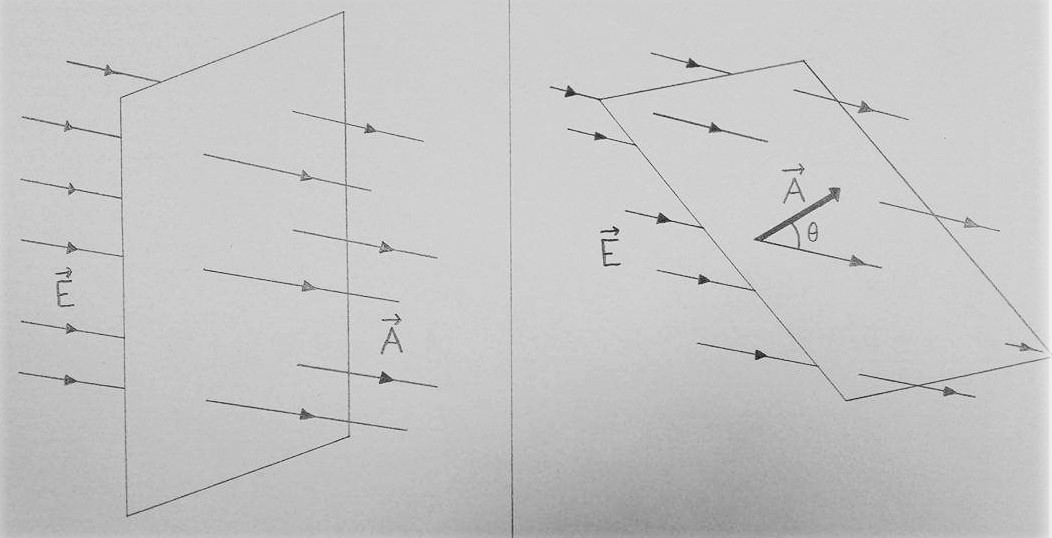
\includegraphics[scale=0.5]{../Vildledning/Schematics/vinkelflux.jpg}
\caption{Figur Vinkelflux}
\end{figure}

Gauss's lov angiver ikke kun den elektriske flux, men den kan benyttes til at beregne den flux, der forløber over et bestemt areal. Derved skal vi integrere i forhold til overfladen, samt at vektor A skal ganges med en faktor d, så vi får $\Phi = \int \vec{E} \bullet d \vec{A}$, som igen kan skrives som $\Phi = \int E \cdot dA \cdot cos(\theta)$. Herefter tager Gauss relation til det cirkulære felt omkring en positiv ladning. A bliver i denne sammenhæng formlen for en kugles overflade $4 \pi r^2$, mens integralet ophæves, da vi nu omtaler hele overfladen igen. Herfra får vi: $\Phi = E \cdot 4 \pi r^2$

Det elektriske felt E er også angivet til at være $\frac{kq}{r^2}$. Ud fra dette får vi den elektriske flux til: $\Phi = \frac{kq}{r^2} \cdot 4 \pi r^2 = 4 \pi k q$. k er derudover defineret som $\frac{1}{4 \pi \epsilon_0}$, hvilket vi kan indsætte i forrige formel, hvorved vi får: $\frac{4 \pi q}{4 \pi \epsilon_0} = \frac{q}{\epsilon_0}$.

q angiver den omkransede ladning for en lukket overflade. Derved kan vi opskrive Gauss's lov til følgende:

\centerline{$\oint \vec{E} \bullet d \vec{A} = \frac{q}{\epsilon_0}$}

\begin{itemize}
\item Elektromagnetisme
\begin{itemize}
\item Ampère's lov
\end{itemize}
\end{itemize}
Ampère's lov beskriver relationen mellem magnetiske feltstyrker og størrelsen af en jævn strøn gennem en ledning givet over længden l. Ampère tager udgangspunkt i, hvis man befinder sig ved ledningens center og følger magnetfeltet, som omkredser ledningen. Her er magnetfeltets styrke defineret ved vektoren $\vec{B}$, og et definerede linjestykke af magnetfeltets længde angives som $\vec{dl}$. For at beregne den jævne strøm gennem ledningen, skal vi tage integralet af de to vektorer prikket sammen. Herved beskrives Ampére's lov:

\centerline{$\oint \vec{B} \bullet \vec{dl} = \mu_0 I$}

Vektor $\vec{B}$ er angivet ved $\frac{\mu_0 I}{2 \pi r}$, da vi arbejder med et cirkelformet magnetfelt. Derudover er det lukkede integrale af $\vec{dl}$ den totale længde af cirkelperiferien angivet ved $2 \pi r$. Produktet mellem disse vil dermed blive $\mu_0 I$, som vi ser på højre side af Ampére's lov.


\begin{itemize}
\item Faraday's lov
\end{itemize}
En af de begreber, som elektromagnetisme beskriver, er induktion af spænding ved hjælp af magnetisme. Før vi ser på Faraday's lov, skal vi kende begrebet magnetisk flux. Magnetisk flux ligner til delt elektrisk flux, som beskrevet tidligere. Her tager man integralet over det magnetiske felt prikket med et bestemt overfladeareal: $\Phi_B = \int \vec{B} \bullet \vec{dA}$

En induseret strøm opstår ikke fra den magnetiske flux alene, men ved en ændring i den magnetiske flux. Dette betyde, at der bliver induseret spænding, hvis der sker en ændring af magnetfeltets styrke, den påvirkede overflades størrelse eller vinklen for, hvordan det magnetiske felt går gennem den pågældende overflade.

Faraday benytter den magnetiske flux til at beskrive den inducerede spænding ved:

\centerline{$\varepsilon = -1 \cdot \frac{d \Phi_B}{dt}$}

Ændringen af den magnetiske flux optræder ofte modsat af den inducerede spænding, så derfor ganger Faraday en faktor -1 på det differentierede udtryk af den magnetiske flux. Den magnetiske flux kan også beskrives som $\vec{B} \bullet \vec{A}$ eller $B \cdot A \cdot cos(\theta)$.
\begin{itemize}
\item Maxwell's ligninger (Forbindelse mellem Faraday og Ampère)
\end{itemize}
Ved trådløs opladning arbejder man med at omdanne elektrisk flux til magnetisk flux gennem spolen ved transmitteren, hvorefter den magnetiske flux igen skal omdannes til en elektrisk flux ved modtageren. For at beskrive hvordan elektriske felter omdannes til magnetisk flux, så skal vi se nærmere på Ampére's lov. Herefter kan overgangen fra magnetfelt til elektrisk flux beskrives gennem Faraday's lov. Til slut kan vi se på Maxwell's ligninger, som bygger videre på Ampère's og Faraday's love, hvorved vi kan skabe en sammenhæng.

Maxwell indså, at der måtte foretages modifikationer for Ampére's lov, hvis der skulle kunne skabes symmetri med Faraday's lov. Ved Maxwell's ligninger er Faraday's lov opgivet som det lukkede linjeintegrale af det magnetiske felt, som er lig det negative differentiale af den magnetiske flux i forhold til tid: $\oint \vec{E} \bullet \vec{dl} = -1 \cdot \frac{d \Phi_B}{dt}$.

Herefter kan vi kaste et blik på Maxwell's modificerede udgave af Ampère's lov. Maxwell har her udbygget formlen, så der skabes en symmetri med Faraday's lov. Derved bliver Ampère's lov omskrevet til, at det lukkede linjeintegrale af det magnetiske felt er lig den elektriske spænding lagt sammen med differentialet af den elektriske flux i forhold til tiden, hvorpå der er ganget en faktor bestående af produktet mellem permeabilitetskonstanten og permittivitetskonstanten: $\oint \vec{B} \bullet \vec{dl} = \mu_0 \cdot I + \mu_0 \epsilon_0 \cdot \frac{d \Phi_E}{dt}$.

Grunden til, at Maxwell udbygger Ampère's lov, er, at loven kun er gældende for, at en stabil strøm er med til at danne en magnetisk flux. For at skabe symmetri med Faraday, udformede Maxwell sin teori om, at elektrisk flux også er gældende for at danne magnetisk flux ved en ustabil strøm. Derved er udtrykket $\mu_0 \epsilon_0 \cdot \frac{d \Phi_E}{dt}$ tilføjet til det oprindelige udtryk.
\newpage
\section{Basis-begreber??}
\subsection{Mikrobølger}
En metode man kan bruge til at sende energi trådløst er ved hjælp af mikrobølger hvor man så omdanner den elektriske energi til mikrobølger og så sender dem var en PTU (Power Transmitter Unit) og til PRU (Power Receiver Unit). Hvor ved at man så omdanner mikrobølgerne tilbage til elektrisk strøm. Den typiske frekvens man bruger ligger mellem 300 MHZ og 300 GHZ. Mikrobølger har en fordel i form af at de kan sammen med at de sender energi, så kan de også bruges til at sende information, altså de kan bruges til kommunikation.  Det er ikke en mulighed som bliver brugt særlig ofte, da der kan ske mutationer hvis man er udsat for enten for hård stråling eller hvis man ofte bliver udsat for strålingen. Der er så stor fare at The Federal Communications Commission (FCC) har beslaglagt de stærke transmittere. Det er en af grundene til at man ikke bruger dem i bl.a. mobilopladere. FCC har lagt restriktioner på laderne til at må være på maks 4 W.
\subsection{Elektromagnetisme}
Elektromagnetisme er i sin enkelthed meget simpel. Elektromagnetisme virker på den måde at man har et materiale som man gør magnetisk ved hjælp af at sende en elektrisk strøm igennem. Ved at man gør det vender atomerne sig så de følger strømmen, og man får derved skabt 2 modstående poler som tiltrækker negativt eller positivt ladede partikler. En af fordele ved elektromagnetisme er at man selv kan sørge for hvornår et materiale skal være magnetisk og hvornår materialet ikke skal være magnetisk, ved at det er elektrisk kan man også bruge det til at vende polerne. Hvis man bruger jævnstrøm kan man holder polerne på plads, og hvis man bruger vekselstrøm kan man få polerne til at skifte retning kan man styre magnetiske felter. Og det gør at man kan bruge dem som motor. Når man snakker om elektromagnetisme bliver man også nød til at snakke om induktion. Induktion sker når man bruger magnetisme til at vende polariteten på fx en gryde eller mobil. Man kan vende polariteten på en gryde for at gøre gryden varm, altså til at lave mad, men uden faren for at man kan brænde sig på blusset bagefter, da pladen aldrig er blevet varm. Man kan også bruge induktion til hvis man vil lade sin mobiltelefon op, der er efterhånden mange teleselskaber som har gjort deres mobiler klar til at kunne lades op uden at skulle sætte et stik i den ene ende. Det er fx selskaber som Apple, Samsung, Huawei osv. Måden telefonen lader er at telefonen ligges på en flade hvor der er et magnetisk felt, som telefonen bryder og når det sker begynder telefonen lige som gryden at modtage energi, som den omdanner til elektrisk energi.
\subsection{Spoler}
I dette afsnit er der planlagt, at blive snakket om spoler. Både i forhold til vores kredsløb i plecs, samt hvordan det bedst kan benyttes til "wireless power transfer".
\newpage
\subsection{Opbygning af kredsløb??}
\begin{figure}[htbp]
	\centering
	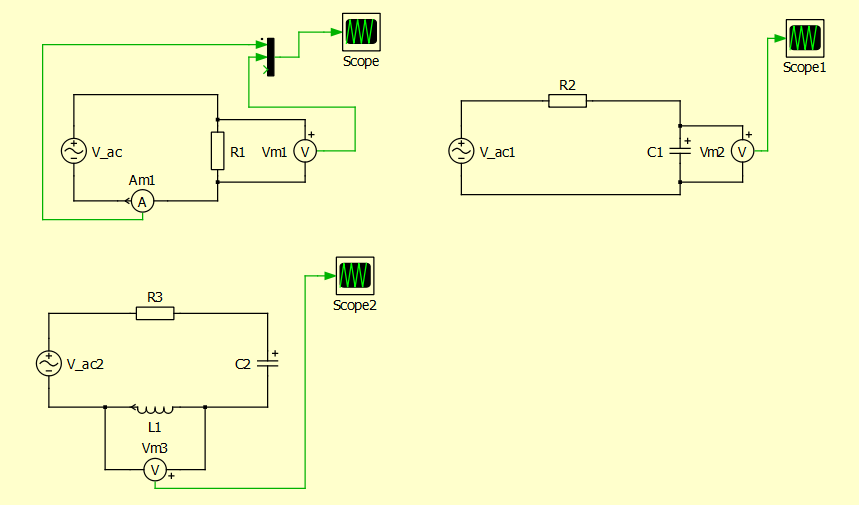
\includegraphics[width=1\textwidth]{../Vildledning/Schematics/Eks1_LCR.png}
	\caption{LCR-Kredsløb}
\end{figure}

Hvor:
\begin{table}[H]
	\begin{tabular}{l|l}
	$R$     & Resistans [\si \ohm] \\
	$V_{ac}$ 	   &  Generator[\si Volt] \\
	$A$ 	   & Ampere-meter [\si Ampere] \\
	$V$			& Volt-meter [\si Volt]
	\end{tabular}
\end{table}

\subsection{Qi}
For at få implementeret trådløs opladning, så skal produkterne overholde bestemte systemkrav, for at opladningen skal kunne fungere optimalt eller overhovedet fungere.

Wireless power consortium er en samlet organisation af forskellige virksomheder, som arbejder med trådløs opladning indenfor mange forskellige produkter. De har igennem denne organisation opsat det, de kalder Qi-standarderne, som beskriver hvilke systemkrav der skal opfyldes, og hvilke dele der skal implementeres i produkterne, før de er kompatible til trådløs opladning.

For at en trådløs opladning kan finde sted, skal der være en transmitter, der udsender strømmen, mens der i modsatte ende skal være en modtager, der opfanger strømmen og oplader produktet. For at produktets opladning skal godkendes af Qi-standarderne, skal transmitteren indeholde en brugerflade, som kan koples sammen med alle godkendte modtagere. Derudover skal modtageren kunne sende oplysningerne omkring opladningen tilbage til transmitteren, så den modtager data, den kan bearbejde.
\end{document}